\chapter{User manual}
\section{Install web component}
To install the application simply add the script to your HTML file as shown in figure \ref{fig:install}
\begin{figure}[H]
    \centering
    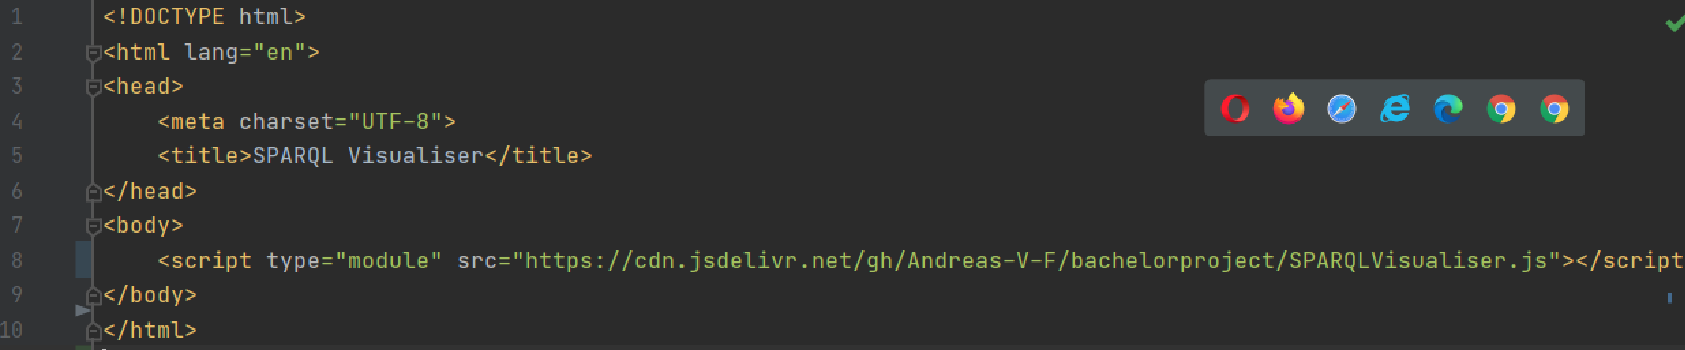
\includegraphics[width=1\textwidth]{figures/install.pdf}
    \caption{Installation of the software}
    \label{fig:install}
\end{figure}
\section{Using the software}
Nodes are draggable by holding the left mouse button down. 
\subsection{Add node}
To add a node to the visualisation click the Add node tool. A popup will be shown, see figure \ref{fig:user-add}. Fill out the name and whether the node should be bounded or not. A bounded variable will be shown as blue while an unbounded variable will be red.

\begin{figure}[H]
    \centering
    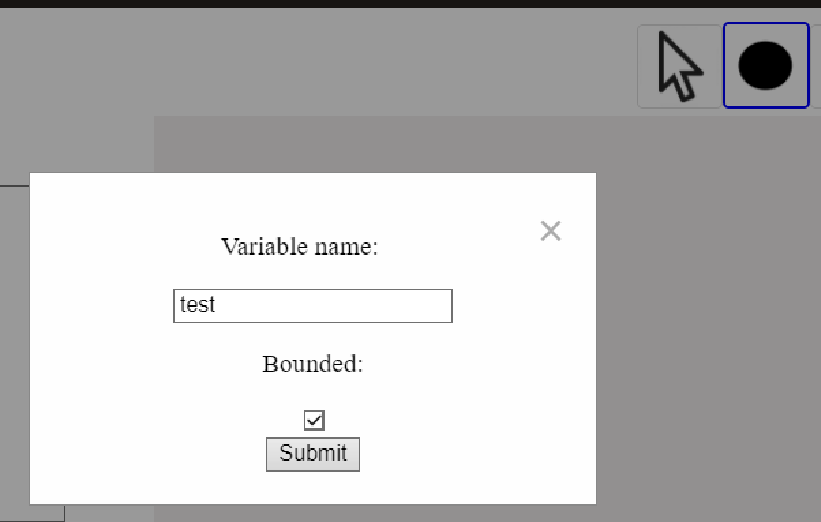
\includegraphics[width=1\textwidth]{figures/add-node-user.pdf}
    \caption{Adding a node}
    \label{fig:user-add}
\end{figure}
\subsection{Draw line}
Select the connect nodes tool. Now click two nodes which are not already connected. Fill out the predicate name, see figure \ref{fig:user-line}. As well as the now added line, you will see an update to the text area in the top left.
\begin{figure}[H]
    \centering
    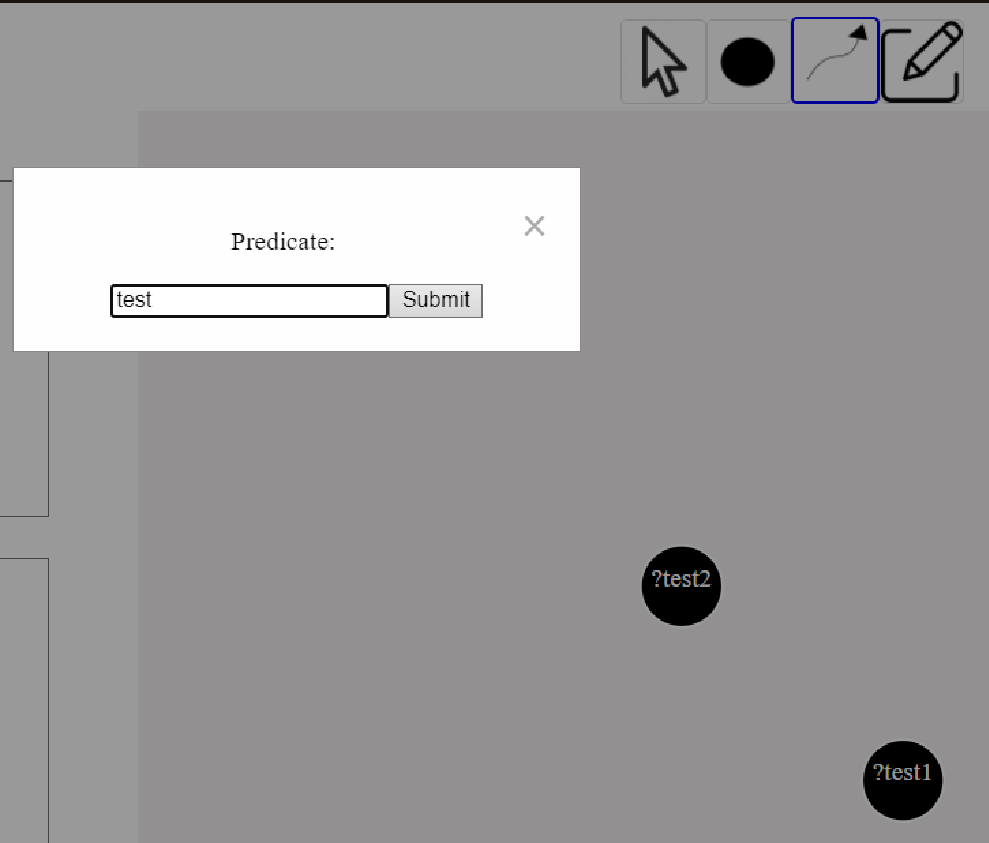
\includegraphics{figures/add-line-user.pdf}
    \caption{Adding a line}
    \label{fig:user-line}
\end{figure}
\subsection{Write query}
Go to the text area in the top left. Fill out a query. Press the run button to run the parser. If your query is insufficient, an error message will show in the text area below, figure \ref{fig:user-write-error}. Use this error message to figure out how to correct your query. On a successful parse, your query will be shown in the visualisation, figure \ref{fig:visual-success}.
\begin{figure}[H]
    \centering
    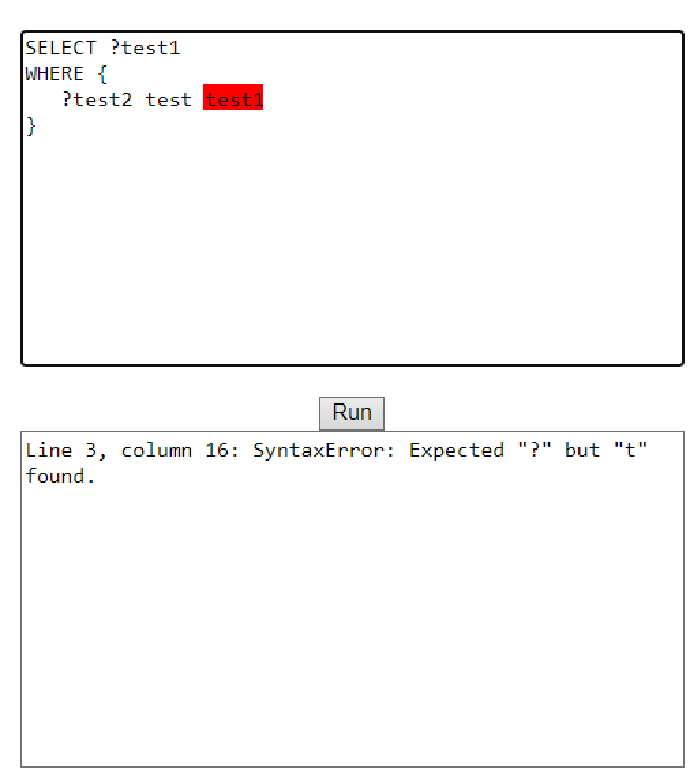
\includegraphics[width=0.6\textwidth]{figures/user-write-error.pdf}
    \caption{Caption}
    \label{fig:user-write-error}
\end{figure}

\begin{figure}[H]
    \centering
    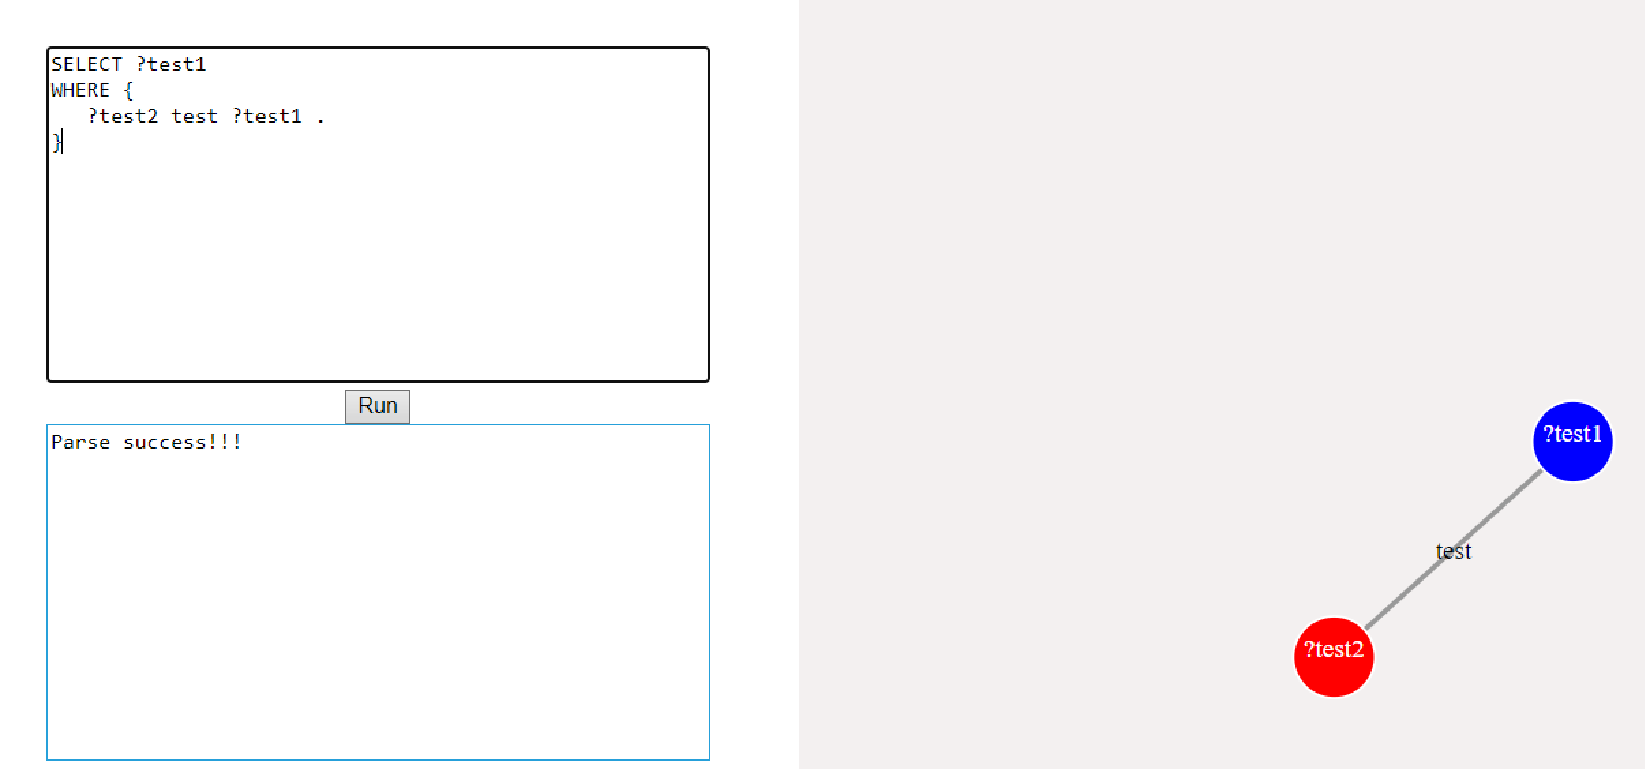
\includegraphics[width=1\textwidth]{figures/visual-query-succ.pdf}
    \caption{Caption}
    \label{fig:visual-success}
\end{figure}

\subsection{Selection}
Click on the select tool. When clicking on either a node or a line, they will be added to the selection. Selected elements are shown as black, figure \ref{fig:user-select}. If you want to delete selected elements, press the delete key on the keyboard.
\begin{figure}[H]
    \centering
    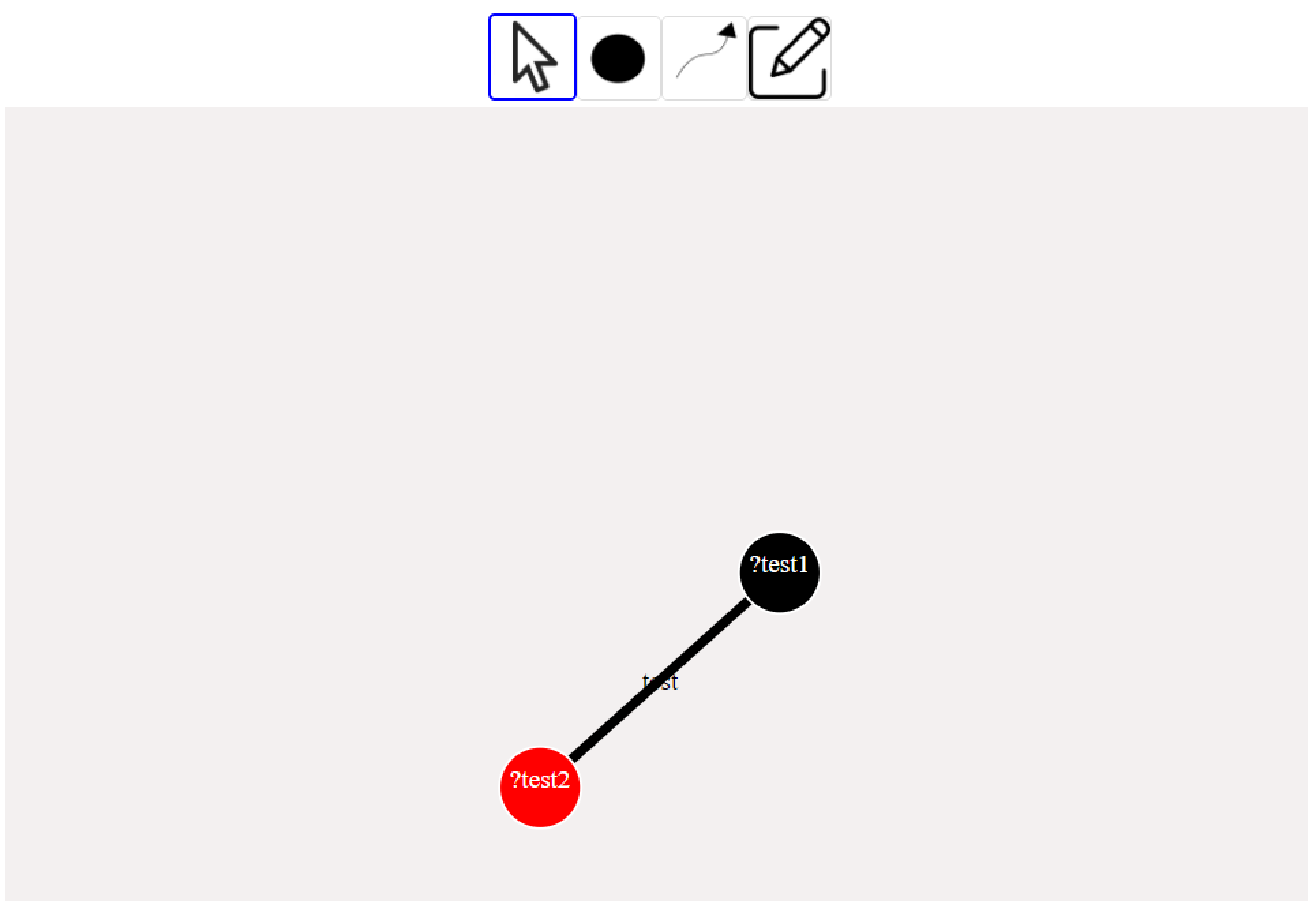
\includegraphics{figures/user-select.pdf}
    \caption{A showcase of }
    \label{fig:user-select}
\end{figure}
\subsection{Editing}
Choose the edit tool. Click either a node or a line. A popup will occur with the selected elements information\ref{fig:user-edit}. Change the information and press submit to edit.
\begin{figure}[H]
    \centering
    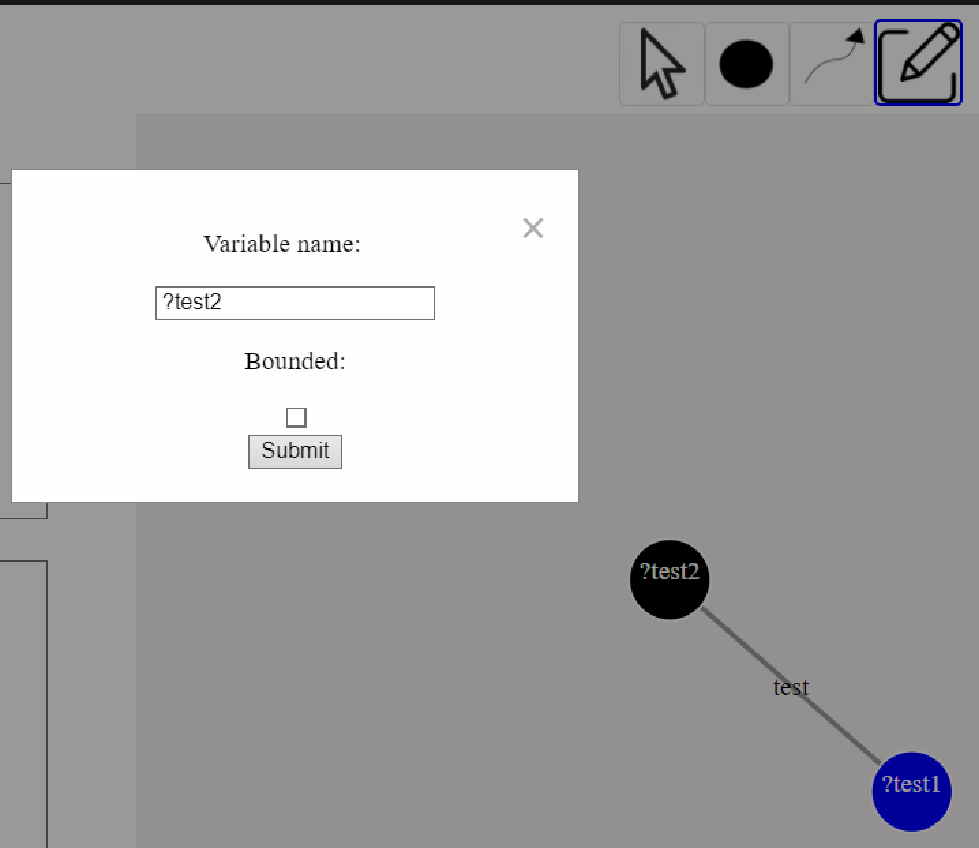
\includegraphics{figures/user-edit.pdf}
    \caption{The edit tool in action}
    \label{fig:user-edit}
\end{figure}
\subsection{Downloading and uploading}
To download the visualisation click the download button. A JSON file will be downloaded to your computer. To load the JSON file, use the choose file button and locate the JSON file. Now click upload. The visualisation and textual area shall be updated to resemble your previously download JSON.